\documentclass[twoside, a4paper]{report}

\usepackage[ngerman]{babel}
\usepackage[margin=2cm]{geometry}
\usepackage{float, mathtools, tabularx, booktabs, empheq, graphicx}

\graphicspath{{Grafiken/}}

% \usetikzlibrary{arrows.meta}
% \tikzset{>=latex}

% \usetikzlibrary{angles, arrows}
% \pgfplotsset{
%   width=7cm,
%   grid = major,
%   axis lines = center,
% }

\title{Statistik Formelsammlung}
\author{Tim Hilt \and Emil Slomka}
\date{30. Dezember 2019}

% \setlength{\extrarowheight}{12pt}
\begin{document}

\maketitle
\tableofcontents

\part{Beschreibende Statistik}

\chapter{Kombinatorik und Wahrscheinlichkeitsrechnung}

\section{Kombinatorik}

\subsection{Permutation}

\begin{center}
  \begin{tabular}{lc}
    \toprule
    Permutation ohne Wiederholung: & \(n\!\)\\
    \midrule
    Permutation mit Wiederholung: & \(\displaystyle{\frac{n!}{k_1! \cdot k_2! \cdot \cdots \cdot k_s!}}\)\\
    \bottomrule
  \end{tabular}
\end{center}

\section{Kombination und Variation}

Kombinationen werden verwendet, wenn \textbf{nur einige} der Elemente in einer Menge angeordnet werden sollen. Permutationen hingegen ordnen \textbf{alle} Elemente an.

\begin{figure}[H]
  \centering
  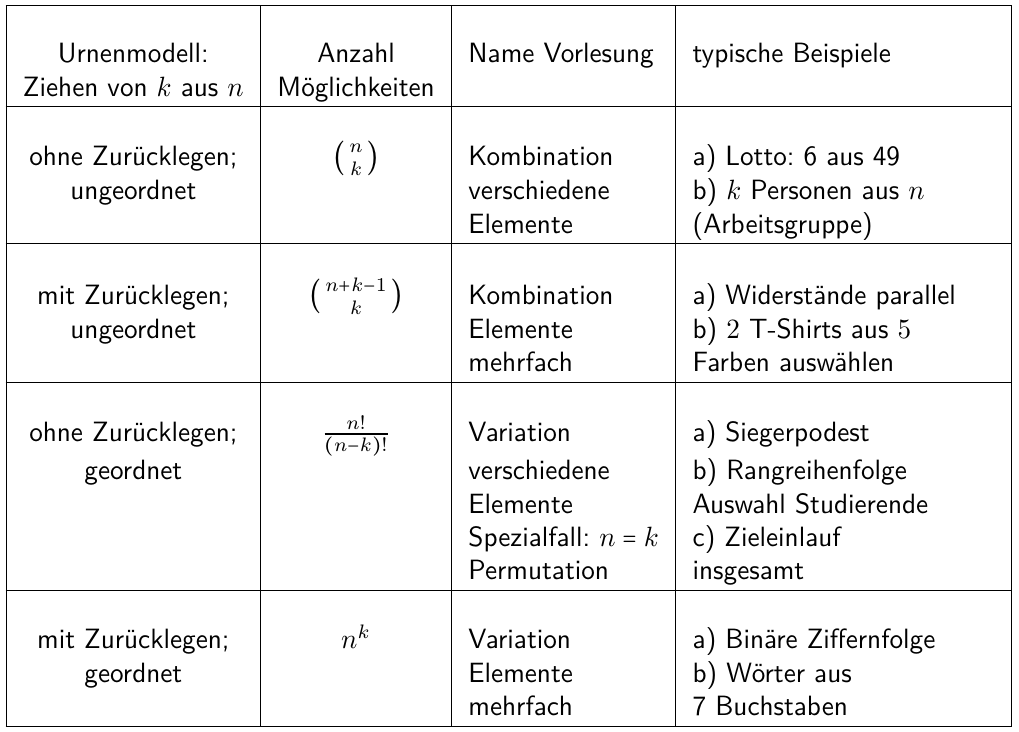
\includegraphics[width=11cm]{Grafiken/Kombinatorik}
\end{figure}

\section{Wahrscheinlichkeitsrechnung}

\subsection{Wahrscheinlichkeitsverteilungen}

\begin{figure}[H]
  \subsubsection{Allgemeine Form}
  \textbf{Dichtefunktion:}

  Funktion, bei der auf der \(x\)-Achse alle Elemente mit der auf der \(y\)-Achse aufgetragenen Wahrscheinlichkeit gezeichnet sind. Es ergibt sich ein Säulendiagramm.

  \textbf{Verteilungsfunktion:}
  \[F(x) = P(X \leq x) = \sum_k^x(k \cdot P(X=k))\]
  \textbf{Erwartungswert:}
  \[E(X) = \mu = \sum_k k \cdot P(X=k)\]
  \textbf{Varianz}
  \[\operatorname{Var}(X) = \sigma^2 = \sum_k {(k^2 \cdot P(X=k) )} - \mu^2\]
\end{figure}

\begin{figure}[H]
  \subsubsection{Hypergeometrische Verteilung}
Beschreibung: Ziehen ohne Zurücklegen $\rightarrow$ Wahrscheinlichkeit verändert sich im Verlauf des Experiments

  Es müssen folgende Variablen (bis auf \(k\)) gegeben sein:

  \begin{tabular}{ll}
    \toprule
    \(N\) & Anzahl aller Elemente\\
    \(M\) & Anzahl Elemente mit bestimmter Eigenschaft\\
    \(n\) & Anzahl Elemente in der Stichprobe\\
    \(k\) & Anzahl Elemente aus der Stichprobe, die das Merkmal aufweisen sollen\\
    \bottomrule
  \end{tabular}

  \textbf{Dichtefunktion:}
  \begin{align*}
    X &\sim H(n, N, M)\\[1em]
    P(X = k) &= \frac{\binom{M}{k}\binom{N-M}{n-k}}{\binom{N}{n}}
  \end{align*}
  \textbf{Verteilungsfunktion:}
  \[F(x) = P(X \leq x) = \sum_{k=0}^x\operatorname{H}(k,n,N,M)\]
  \textbf{Erwartungswert:}
  \[E(X) = \mu = n \cdot \frac{M}{N}\]
  \textbf{Varianz:}
  \[\operatorname{Var}(X) = \sigma^2 = n \cdot \frac{M}{N} \left(1 - \frac{M}{N}\right) \frac{N - n}{N - 1}\]
\end{figure}

\begin{figure}[H]
  \subsubsection{Binomialverteilung}
Beschreibung: Ziehen \textbf{mit} zurücklegen $\rightarrow$ Wahrscheinlichkeit bleibt während dem Experiment gleich

  Es müssen folgende Variablen gegeben sein:

  \begin{tabularx}{\textwidth}{lX}
    \toprule
    \(p\) & Anteil der Elemente/ Wahrscheinlichkeit beim Ziehen \textbf{eines} Elementes aus der Grundgesamtheit\\
    \(n\) & Anzahl Elemente in der Stichprobe\\
    \(k\) & Anzahl Elemente aus der Stichprobe, die das Merkmal aufweisen sollen\\
    \bottomrule
  \end{tabularx}

  \textbf{Dichtefunktion:}
  \begin{align*}
    X &\sim \operatorname{B}(n,p)\\[1em]
    P(X = k) &= \binom{n}{k}p^k{(1 - p)}^{n-k}
  \end{align*}
  \textbf{Verteilungsfunktion:}
  Hier müssen die einzelnen Dichtefunktionen berechnet werden
  \[F(x) = P(X \leq x) = \sum_{k=0}^x\operatorname{B}(k,n,p)\]
  \textbf{Erwartungswert:}
  \[E(X) = \mu = n \cdot p\]
  \textbf{Varianz:}
  \[\operatorname{Var}(X) = \sigma^2 = n \cdot p \cdot (1 - p)\]
  \textbf{Annäherung der Hypergeometrischen Verteilung durch Binomialverteilung:}\\
  Falls \(\frac{n}{N} \leq 0.1\) kann der Parameter \(p\) durch \(p = \frac{M}{N}\) angenähert werden.
\end{figure}

\begin{figure}[H]
  \subsubsection{Poissonverteilung}
  Beschreibung: Gegeben ist ein Durchschnittswerts (\textit{Erwartungswert}) \(\lambda\) pro einer gewissen Einheit (z.B. im Durchschnitt 3 Anrufe in 5 Minuten). Die Poissonverteilung soll berechnen, wie groß die Wahrscheinlichkeit ist einen anderen Wert \(k\) als Ergebnis zu erhalten.\\
  \textbf{Dichtefunktion:}
  \begin{align*}
    X & \sim \operatorname{Po}(\lambda)\\[1em]
    P(X = k) & = \frac{\lambda^k}{k!}e^{-\lambda}
  \end{align*}
  \textbf{Verteilungsfunktion:}
  \[F(x) = P(X \leq x) = \sum_{k=0}^x\operatorname{Po}(k,\lambda)\]
  \textbf{Erwartungswert:}
  \[E(X) = \mu = \lambda\]
  \textbf{Varianz:}
  \[\operatorname{Var}(X) = \sigma^2 = \lambda\]
  \textbf{Annäherung der Binomialverteilung durch Poissonverteilung:}\\
  Wenn \(n\) groß und \(p\) klein ist (\(n \geq 30, p \leq 0.1\)) kann der Parameter \(\lambda\) durch \(\lambda = n \cdot p\) angenähert werden.
\end{figure}

\begin{figure}[H]
  \subsubsection{Geometrische Verteilung}
  Beschreibung: Gegeben ist die Wahrscheinlichkeit für einen Erfolg (\(p\), Misserfolg \(q = 1-p\)). Die geometrische Verteilung berechnet die Wahrscheinlichkeit dafür, dass genau \(k\) Versuche benötigt werden um zum ersten Erfolg zu kommen; dass man also \textbf{beim} \(k\)-ten Versuch Erfolg hat.\\
  \textbf{Dichtefunktion:}
  \[P(X=k) = p \cdot { (1-p) }^{k-1}\]
  \textbf{Verteilungsfunktion:}
  \[P(X \leq k) = 1 - { (1-p) }^k\]
  \textbf{Erwartungswert:}
  \[E(X) = \mu = \frac{1}{p}\]
  \textbf{Varianz:}
  \[\operatorname{Var}(X) = \sigma^2 = \frac{1-p}{p^2}\]
\end{figure}

\subsubsection{Quantile und Zufallsstreubereich der Normalverteilung}

Quantile berechnen einen bestimmten Prozentsatz der Fläche unter der Verteilungsfunktion einer normalverteilten Zufallsvariable.

Bsp.\ das 95\% Quantil wird geschrieben als
\begin{empheq}[box=\fbox]{align*}
  q_{0.95} = \mu\ + z_{0.95} \cdot \sigma\
\end{empheq}

Das bedeutet, dass 95\% der Werte unterhalb des Wertes \(q_{0.95}\) liegen.

Die Werte für \(z_m\) sind tabelliert, können jedoch auch mit dem Taschenrechner (mit $\mu=0$ und $\sigma=1$) berechnet werden:

\begin{center}
  \begin{tabular}{llllllll}
    \toprule
    \(m\) & \(0.8\) & \(0.9\) & \(0.95\) & \(0.975\) & \(0.99\) & \(0.995\) & \(0.999\)\\
    \(z_m\) & \(0.842\) & \(1.282\) & \(1.654\) & \(1.960\) & \(2.326\) & \(2.576\) & \(3.090\)\\
    \bottomrule
  \end{tabular}
\end{center}

Der Zufallsstreubereich (ZSB) Ist ein Intervall, das zwei Quantile berechnet. ZSBs können nach unten, nach oben oder zweiseitig beschränkt sein. Der Zufallsstreubereich kann für ein gegebenes \(\mu\) oder für den arithmetischen Mittelwert \(\overline{X}\) eines gegebenen Datensatzes berechnet werden.

Es sei \(p\) die gegebene Wahrscheinlichkeit/die gewünschte Fläche unter der Verteilungsfunktion für das Quantil oder den ZSB.\ Wir definieren \(\alpha\) als den Kehrwert \(\mathbf{\alpha = 1 - p}\) von \(p\).

Soll nun ein ZSB berechnet werden so passiert dies über die Formeln:

\begin{center}
  \begin{tabular}{lrcl}
    \toprule
    Nach oben beschränkt & \((-\infty\ ;\ q_{1-\alpha}]\) & \(=\) & \((-\infty\ ;\ \mu + z_{1-\alpha} \cdot \sigma]\)\\
    Nach unten beschränkt & \([q_{\alpha}\ ;\ \infty)\) & \(=\) & \([\mu - z_{1- \alpha} \cdot \sigma\ ;\ \infty)\)\\
    Beidseitig beschränkt & \([q_{\frac{\alpha}{2}}\ ;\ q_{1-\frac{\alpha}{2}}]\) & \(=\) & \([\mu - z_{1-\frac{\alpha}{2}} \cdot \sigma\ ;\ \mu + z_{1-\frac{\alpha}{2}} \cdot \sigma]\)\\
    \bottomrule
  \end{tabular}
\end{center}

Auch hier kann der Taschenrechner eingesetzt werden (InvNormal). Hier sind die Werte \textbf{Area, $\mu$ und $\sigma$} verlangt. $\mu$ und $\sigma$ sind meist in der Aufgabenstellung gegeben, für Area muss:

\begin{center}
  \begin{tabular}{llc}
    \toprule
    einseitiger Grenzwert: &&\\
    \midrule
                           & nach oben beschränkt: & \(p\)\\
                           & nach unten beschränkt: & \(\alpha\)\\
    \midrule
    zweiseitiger Grenzwert: &&\\
    \midrule
                           & untere Grenze: & \(\frac{\alpha}{2}\)\\
                           & obere Grenze: & \(1-\frac{\alpha}{2}\)\\
    \bottomrule
  \end{tabular}
\end{center}

Ist ein Datensatz mit \(n\) Elementen gegeben, so ändern sich die Formeln zu:

\begin{center}
  \begin{tabular}{lrcl}
    \toprule
    Nach oben beschränkt & \((-\infty\ ;\ q_{1-\alpha}]\) & \(=\) & \(\left(-\infty\ ;\ \mu + z_{1-\alpha} \cdot \frac{\sigma}{\sqrt{n}}\right]\)\\[1em]
    Nach unten beschränkt & \([q_{\alpha}\ ;\ \infty)\) & \(=\) & \(\left[\mu - z_{1- \alpha} \cdot \frac{\sigma}{\sqrt{n}}\ ;\ \infty\right)\)\\[1em]
    Beidseitig beschränkt & \([q_{\frac{\alpha}{2}}\ ;\ q_{1-\frac{\alpha}{2}}]\) & \(=\) & \(\left[\mu - z_{1-\frac{\alpha}{2}} \cdot \frac{\sigma}{\sqrt{n}}\ ;\ \mu + z_{1-\frac{\alpha}{2}} \cdot \frac{\sigma}{\sqrt{n}}\right]\)\\[1em]
    \bottomrule
  \end{tabular}
\end{center}

Nun muss selbstverständlich für $\sigma$ in der InvNormal-Funktion \(\frac{\sigma}{\sqrt{n}}\) eingegeben werden.

\part{Deskriptive Statistik}

\end{document}

%%% Local Variables:
%%% mode: latex
%%% TeX-master: t
%%% End:
